\documentclass{article}
\usepackage[left=1in, right=1in, top=1in, includefoot]{geometry}%Margin
\usepackage{graphicx}%Package to import images
\usepackage{float}%Package to control float position
\usepackage{amsmath}%Package for equations
%Head and foot
%\usepackage[demo]{graphicx}
\usepackage{subfig}
\usepackage{fancyhdr}
\pagestyle{fancy}
\fancyhead{}
\fancyfoot{}
\fancyfoot[R]{\thepage\ }
\renewcommand{\headrulewidth}{1pt}
\renewcommand{\footrulewidth}{1pt}
\fancyhead[L]{Ruohao Zhang}
\fancyhead[R]{rzhang47@binghamton.edu}
\begin{document}
\title{ECON 634 Homework 4}
\author{Ruohao Zhang}
\maketitle
\thispagestyle{fancy}

%QUESTION 1
\section*{\normalsize{Question 1}}
The firms want to solve the optimization function
\begin{equation*}
\begin{aligned}
&\underset{\{K^d_{t+1},\ N^d_t\}}{\text{max}}
\sum_{t=0}^{\infty}\bigg(\frac{1}{\prod^t_{i=0}r_i}\bigg)\pi(K, \ N; \ w_t, \ r_t) \\
&= \underset{\{K^d_{t+1},\ N^d_t\}}{\text{max}}\sum_{t=0}^{\infty}\bigg(\frac{1}{\prod^t_{i=0}r_i}\bigg)\big[K_t^\alpha N_t^{1-\alpha}-w_tN_t-r_tK_t+(1-\delta)K_t\big] 
\end{aligned}
\end{equation*}
and the first order condition $w.r.t \ K_t$ and $N_t$ will be
\begin{equation*}
\begin{aligned}
&\bigg(\frac{1}{\prod^t_{i=0}r_i}\bigg)\big[\alpha K_t^{\alpha -1}N_t^{1-\alpha}-r_t+(1-\delta)\big]=0 \\
&\bigg(\frac{1}{\prod^t_{i=0}r_i}\bigg)\big[(1-\alpha) K_t^{\alpha}N_t^{-\alpha}-w_t\big]=0. 
\end{aligned}
\end{equation*}
Given $K$ and $N$, these two functions show the factor prices are
\begin{equation*}
\begin{aligned}
&r_t=\alpha K_t^{\alpha -1}N_t^{1-\alpha}+(1-\delta) \\
&w_t=(1-\alpha) K_t^{\alpha}N_t^{-\alpha}.
\end{aligned}
\end{equation*}
%QUESTION 2
\section*{\normalsize{Question 2}}
The households want to solve the optimization function
\begin{equation*}
\begin{aligned}
&v(z_t, \ a_t)=
& &\underset{a_{t+1}}{\text{max}}\frac{(z_tw_t\bar{l}+r_ta_t-a_{t+1})^{1-\sigma}}{1-\sigma}+\beta E_t\big[v(z_{t+1}, \ a_{t+1})\big]. \\
\end{aligned}
\end{equation*}	
%QUESTION 3
\section*{\normalsize{Question 3}}
By setting the grid number $nz=5$ and the scale $m=3$, the grid is  $Z=\begin{pmatrix} 0.5002&0.7072&1.0000&1.4140&1.9993 \end{pmatrix}$ and the invariant distribution of productivity states are $\pi^{inv}(z)=\begin{pmatrix} 0.0145&0.2189&0.5333&0.2189&0.0145\end{pmatrix}$. The aggregate effective labor supply $N^s=1.0338$. 
%QUESTION 4
\section*{\normalsize{Question 4}}
Included in the $Matlab$ code.
%QUESTION 5
\section*{\normalsize{Question 5}}
I set the tolerance level as $0.01$. First, use $\bar{a}=80$ as the upper bound of $a$ so that it will not bound households' saving.  The equilibrium gives interest rate 
$0.99\%$, capital level $K=30.4610$.
\section*{\normalsize{Question 6}}
The interest rate is $0.99\%$. For complete market, $r^{CM}=1.01\%$. So the interest rate in lower than complete market interest rate. The policy functions are shown in figure 1.
\begin{figure}[H]%H means want the figure stay here
	\centering
	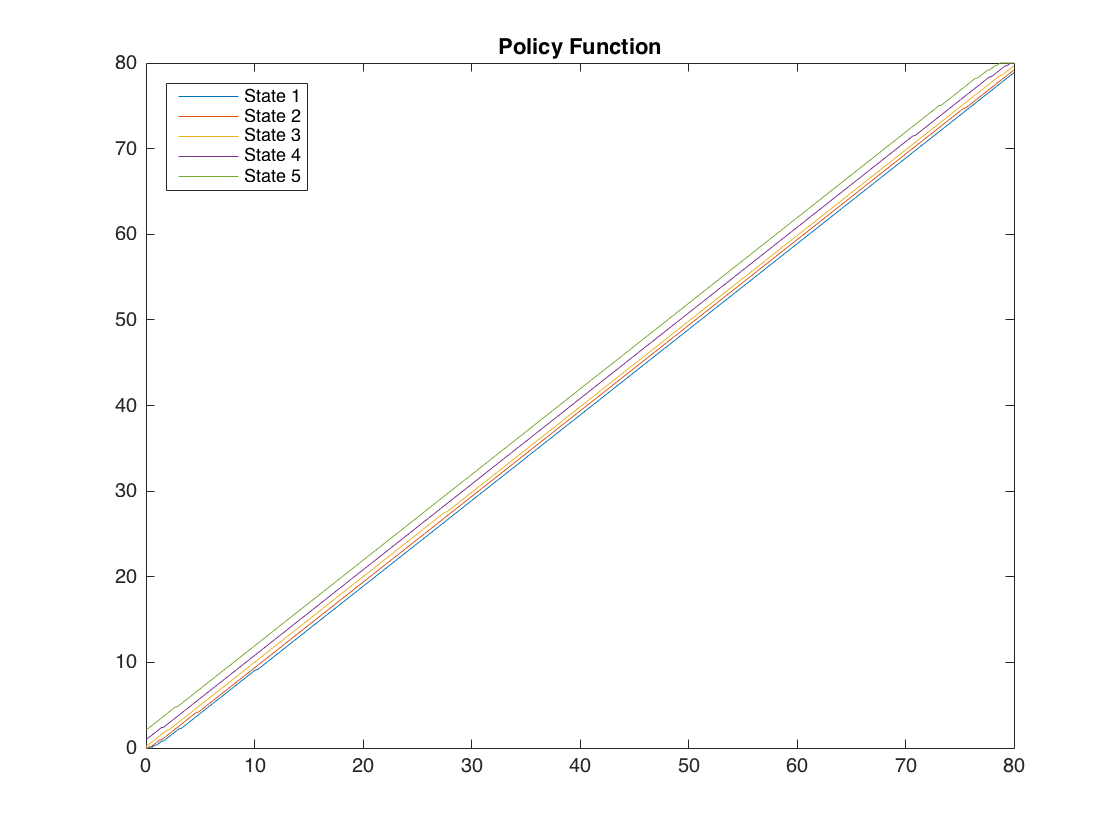
\includegraphics[height=2in]{/Users/ruohaozhang/Documents/Binghamton/ECON634/PS4-RuohaoZhang/Figure/PolicyFn.png}
	\caption[Optional caption]{Policy Function}
	\label{fig:1}
\end{figure}
The Lorenz curve and the wealth distribution are shown below, and I get Gini coefficient $0.22938$. Comparing with Huggett model, Aiyagari model has higher level of equality with lower Gini coefficient, and the wealth distribution gradually increases and suddenly goes to the peak around $K=30$ and decreases gradually to zero. Overall, it is very different from the empirical wealth distribution.
	\begin{figure}[H]%
		\centering
		\subfloat[Lorenz Curve]{{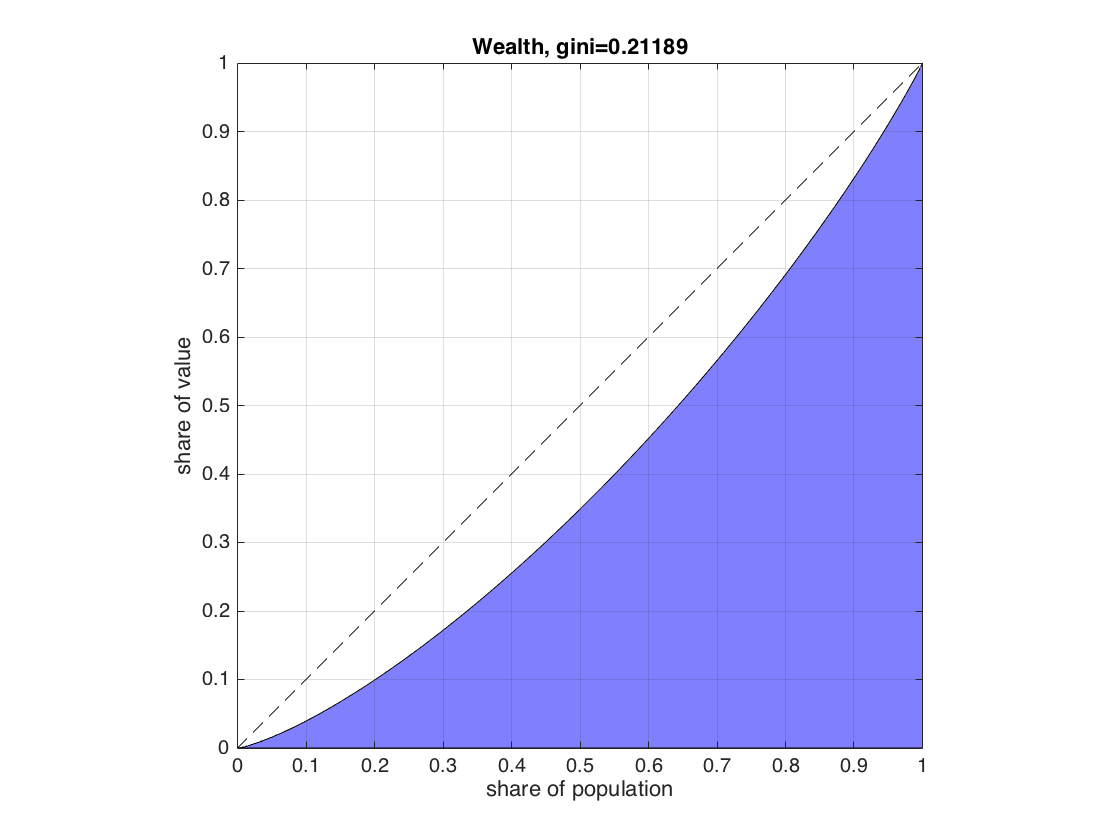
\includegraphics[width=5cm]{/Users/ruohaozhang/Documents/Binghamton/ECON634/PS4-RuohaoZhang/Figure/GiniLorenz.png} }}%
		\qquad
		\subfloat[Wealth Distribution]{{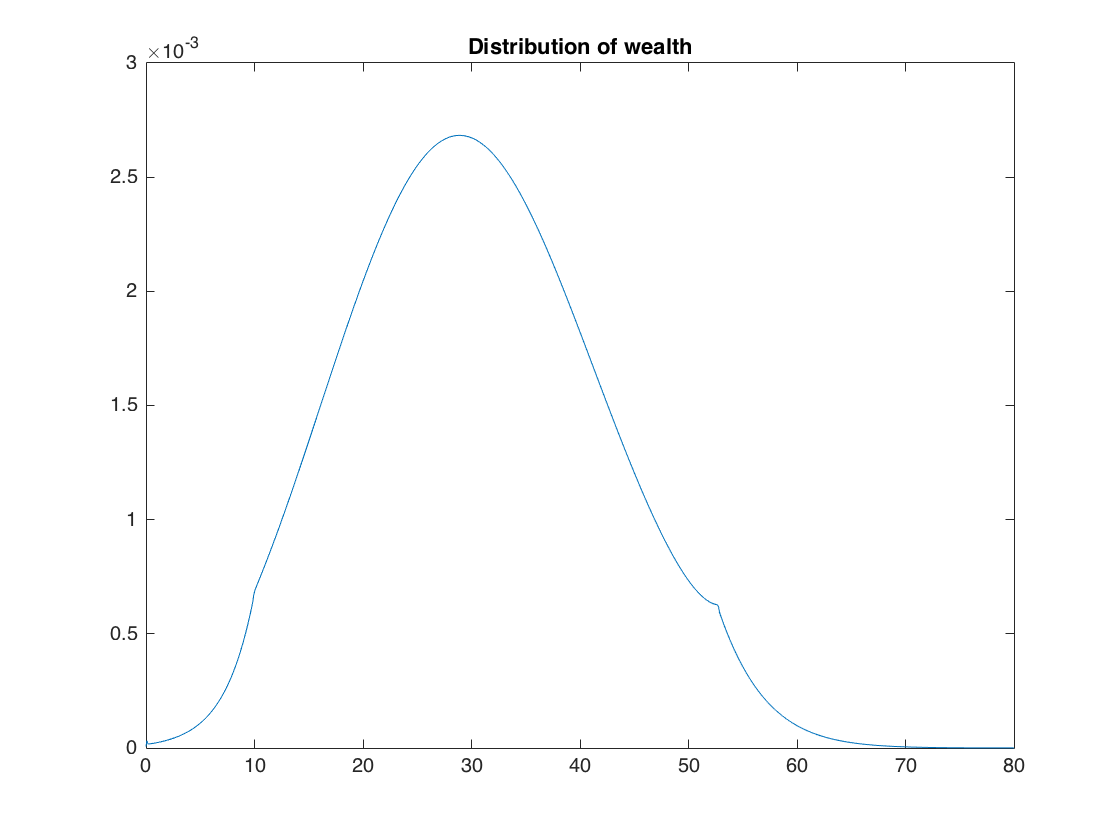
\includegraphics[width=5cm]{/Users/ruohaozhang/Documents/Binghamton/ECON634/PS4-RuohaoZhang/Figure/WealthDist.png} }}%
		\caption{Wealth Distribution}%
		\label{fig:2}%
	\end{figure}
\section*{\normalsize{Question 7}}
Given a fixed $r=1.0099$, the Euler equation for household is
\begin{equation*}
\begin{aligned}
&c_t^{-\sigma}=\beta E\big[c_{t+1}^{-\sigma}r\big]
\end{aligned}
\end{equation*}
The running time is $642.370s$ using VFI only. Using Coase Grid can reduce the running time to $344.740s$, and PFI takes $525.154s$ to get the result. I use the weighted Euler equatoin error to measure the accuacy. The accuracy is $0.00497$ for VFI. After doing the linear interpolation, the error is $0.00495$, which is slightly more accurate. But the running time ($4848.917s$) is much longer. 

















\end{document}